\chapter{Used Mathematical Terminology}

To make this work more integrated, we will briefly remind some mathematical concepts that are used in following chapters. 

\section{Hessian matrix}

Many feature detectors and interest points descriptors use the Hessian matrix. 
The Hessian is a square matrix of the second order partial derivatives of a function. 
Assuming all second partial derivatives exist, for a given function $f\vect{(x_1, x_2, \ldots, x_n)}$ the Hessian looks

\[ H(f) = \left(\begin{array}{c}  
\frac{\partial^2 f}{\partial x_1^2} \frac{\partial^2 f}{\partial x_1 \partial x_2} 
\cdots \frac{\partial^2 f}{\partial x_1 \partial x_n}\\
\frac{\partial^2 f}{\partial x_2 \partial x_1} \frac{\partial^2 f}{\partial x_2^2} 
\cdots \frac{\partial^2 f}{\partial x_2\partial x_n}\\
\cdots \cdots \cdots \\
\frac{\partial^2 f}{\partial x_n \partial x_1} \frac{\partial^2 f}{\partial x_n \partial x_2} 
\cdots \frac{\partial^2 f}{\partial x_n^2}

\end{array}\right)  \]


\section{Integral images}

Later in this work we work with the term of integral images. 
An integral image (also known as summed area table) allows fast and efficient computation over a rectangular area in an image. 
Each pixel represents the sum of all previous pixels above to the left. 
To be more formal, let's see the mathematical formula describing the value of a 
pixel, where \emph{I} is an integral image and $\mathbf{x} = \vect{(x, y)}^{T}$ is a location of a current pixel.

\begin{equation}
 I (\mathbf{x}) = \sum_{i=0}^{i<x} \sum_{j=0}^{j<x} I (i,j)
\end{equation}


An advantage of an integral image is that we are able to construct it with only one pass over the original image. 
Moreover, once we have calculated the integral image, it requires only three integer operations and four memory accesses to calculate the sum 
of intensities inside the region of any size in the picture (see figure 3.1).

\begin{figure}
  \centering{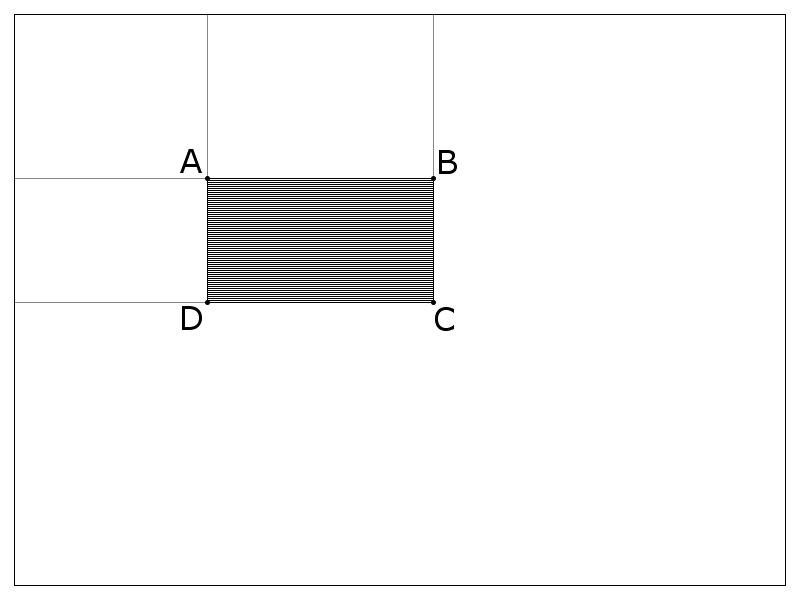
\includegraphics[width=30mm]{img/integral_image.png}}
  \caption{The sum of any rectangular region can be achieved by only three additions.}
\end{figure}
